\subsection{Software Architecture}

\todo[inline]{FIX THE BELOW REFERENCES!!!!}

Since the microcontroller from Energy Micro which this project uses, in turn is
a Cortex microcontroller, the software is based on the CMSIS \ref{CMSIS}
codebase from ARM. The Giant Gecko MCU is supplied with a peripheral Application
Programming Interface (API), called emlib \ref{emlib}, which builds upon CMSIS
and can be used to both initialize and control all attached peripherals. The
structure of the code and programming model is based on how emlib does it. The
code and model have mostly used the emlib API for communicating and controlling
the microcontoller.

\begin{figure}[H]
    \centering
    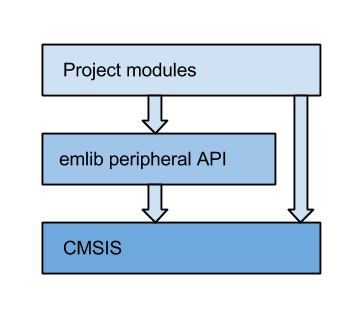
\includegraphics[height=150px]{figures/sw/software-stack.png}
    \caption{The software stack used on the microcontroller}
    \label{fig:software-stack}
\end{figure}


The application code is structured into directories representing each of the
modules or peripherals, whose software was explicity written for this project.
Each directory contains three sub-directories, \textit{inc}, \textit{src} and
\textit{demo}. These sub-directories contain either header files, source files,
or different demos and test programs for each module, respectively. Each module
is typically implemented as a combination of a driver and controller for the
specific peripheral the module is designed for.

\todo[inline]{THE ABOVE PHRASING SUCKS. NEEDS REVISION. -CC}
